\documentclass[11pt,addpoints]{exam}
\usepackage{amsfonts,amssymb,amsmath, amsthm}
\usepackage{enumitem}
\usepackage{graphicx,float}
\usepackage{systeme}
\usepackage{pgf,tikz,pgfplots}
\pgfplotsset{compat=1.15}
\usepgfplotslibrary{fillbetween}
\usepackage{mathrsfs}
\usetikzlibrary{arrows}
\usetikzlibrary{calc}
\usepackage{lipsum}
\usepackage{float}
\usepackage{color,soul}
% \usepackage{times}

\def\testname{CFHS Competitive CS Mid-Term Diagnostic}
\def\examdate{February 2024}

\pagestyle{headandfoot}

\firstpageheader{\testname{}\\ \examdate}{}{KEY}
%\firstpageheadrule

\runningheader{\testname}{}{Page \thepage\ of \numpages}
\runningheadrule

\firstpagefooter{}{}{}
\runningfooter{}{}{}


\begin{document}

\section*{Answers}

\subsection*{Multiple-Choice}

\begin{enumerate}
  \item D
  \item C
  \item C
  \item E
  \item D
  \item A
  \item A
  \item B
  \item D
  \item A
  \item E
  \item A
  \item C
\end{enumerate}

\subsection*{Free Response}

\begin{enumerate}[resume]
  \item {\tt $++$, /, $<<$, $<=$, $!=$, \&, \textasciicircum, |, =}
  \item Bit Table Answer:

\begin{table}[H]
\centering
\begin{tabular}{|l|l|l|}
  \hline
  Type & Bits & Bytes \\ \hline
  boolean & \textcolor{red}{1} & \textcolor{red}{1} \\ \hline
  char & \textcolor{red}{16} & \textcolor{red}{2} \\ \hline
  byte & \textcolor{red}{8} & \textcolor{red}{1} \\ \hline
  short & \textcolor{red}{16} & \textcolor{red}{2} \\ \hline
  int & \textcolor{red}{32} & \textcolor{red}{4} \\ \hline
  long & \textcolor{red}{64} & \textcolor{red}{8} \\ \hline
  float & \textcolor{red}{32} & \textcolor{red}{4} \\ \hline
  double & \textcolor{red}{64} & \textcolor{red}{8} \\ \hline
\end{tabular}
\end{table}

\item Question 16
  \begin{enumerate}[label=(\Alph*)]
    \item $[], [3], [9], [3, 9], [9, 3]$
    \item $[3, 9]$ and $[9, 3]$
  \end{enumerate}

\item Question 17
  \begin{enumerate}[label=(\alph*)]
    \item {\tt return a;} (the last statement in the method.)
    \item This statement will never be reached.
    \item Compiler error.
  \end{enumerate}

\item Question 18
\begin{verbatim}
function BUBBLESORT(ARRAY)							            
    # loop through the array multiple times
    (1) loop INDEX from 0 to size of ARRAY - 1					    
        # consider every pair of elements except the sorted ones
        (2) loop INDEX2 from 0 to size of ARRAY - 2 - INDEX			
            (3) if ARRAY[INDEX2] > ARRAY[INDEX2 + 1] then			
                (4) # swap elements if they are out of order
                TEMP = ARRAY[INDEX2]						    
                ARRAY[INDEX2] = ARRAY[INDEX2 + 1]				
                ARRAY[INDEX2 + 1] = TEMP					    
\end{verbatim}

\item Question 19
\begin{verbatim}
stack A, B

(1) function POP()
  if A is empty
    return nothing or null or -1

  return A.pop()

(2) function PUSH(VALUE)
  while A is not empty
    B.push(A.pop())

  A.push(VALUE)

  while B is not empty
    A.push(B.pop())

\end{verbatim}

\item Question 20
  \begin{enumerate}[label=(\Alph*)]
    \item Part A
      

\tikzset{every picture/.style={line width=0.75pt}} %set default line width to 0.75pt        

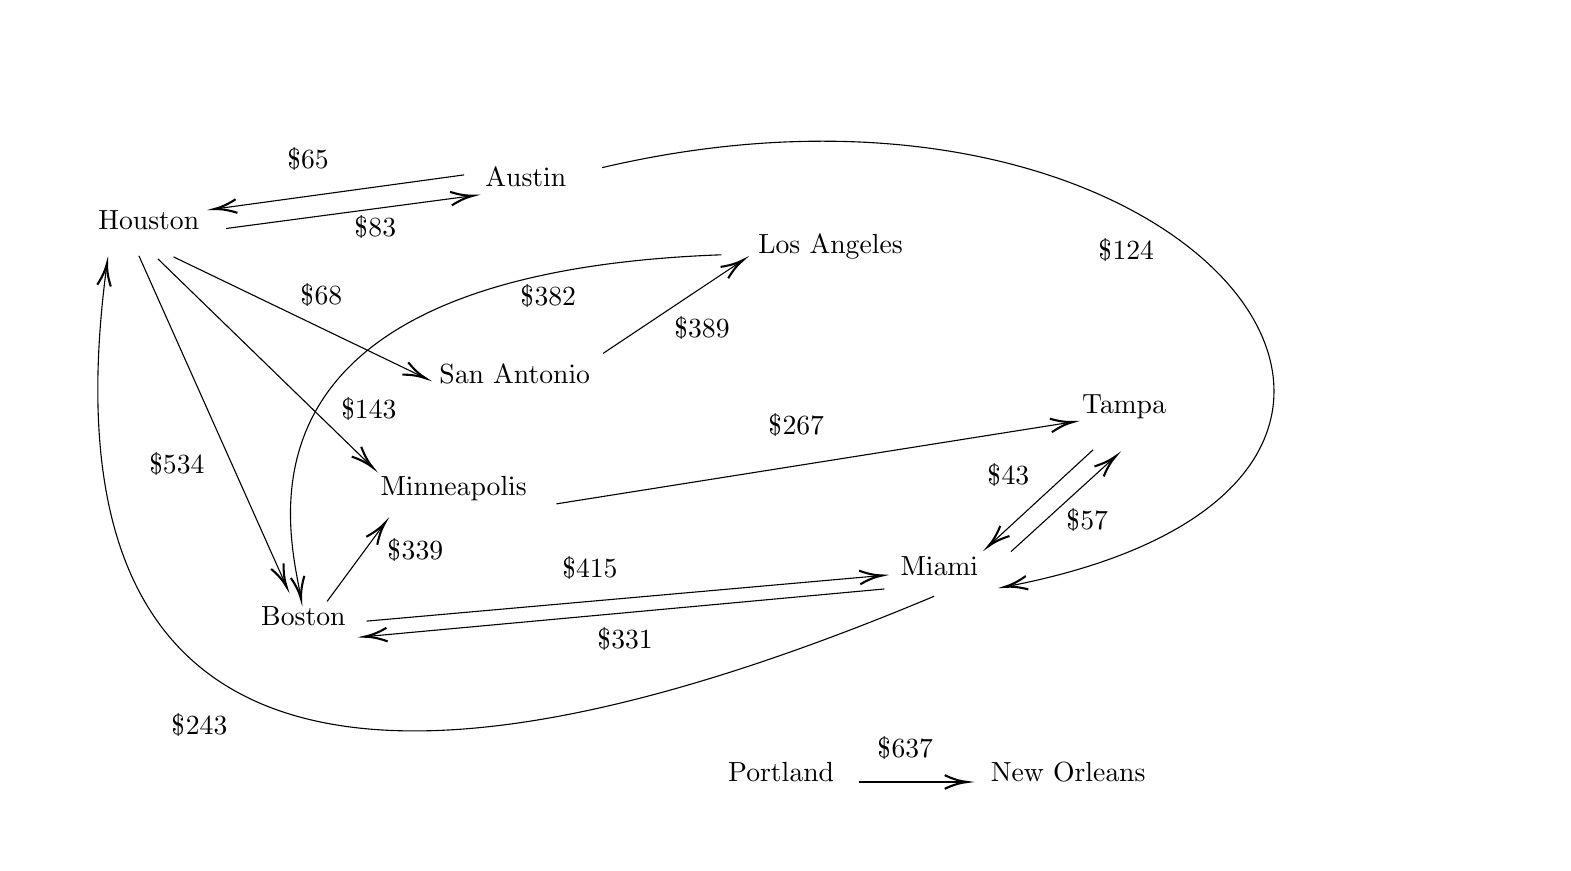
\begin{tikzpicture}[x=0.75pt,y=0.75pt,yscale=-1,xscale=1]
%uncomment if require: \path (0,339); %set diagram left start at 0, and has height of 339

%Straight Lines [id:da5586549096582035] 
\draw    (103,63.5) -- (222.7,121.13) ;
\draw [shift={(224.5,122)}, rotate = 205.71] [color={rgb, 255:red, 0; green, 0; blue, 0 }  ][line width=0.75]    (10.93,-3.29) .. controls (6.95,-1.4) and (3.31,-0.3) .. (0,0) .. controls (3.31,0.3) and (6.95,1.4) .. (10.93,3.29)   ;
%Straight Lines [id:da26174023331430885] 
\draw    (128.33,49.83) -- (245.52,34.26) ;
\draw [shift={(247.5,34)}, rotate = 172.43] [color={rgb, 255:red, 0; green, 0; blue, 0 }  ][line width=0.75]    (10.93,-3.29) .. controls (6.95,-1.4) and (3.31,-0.3) .. (0,0) .. controls (3.31,0.3) and (6.95,1.4) .. (10.93,3.29)   ;
%Straight Lines [id:da2538209687911336] 
\draw    (86.33,63) -- (156.69,220.67) ;
\draw [shift={(157.5,222.5)}, rotate = 245.95] [color={rgb, 255:red, 0; green, 0; blue, 0 }  ][line width=0.75]    (10.93,-3.29) .. controls (6.95,-1.4) and (3.31,-0.3) .. (0,0) .. controls (3.31,0.3) and (6.95,1.4) .. (10.93,3.29)   ;
%Straight Lines [id:da4001782652965149] 
\draw    (243,24) -- (124.48,40.23) ;
\draw [shift={(122.5,40.5)}, rotate = 352.2] [color={rgb, 255:red, 0; green, 0; blue, 0 }  ][line width=0.75]    (10.93,-3.29) .. controls (6.95,-1.4) and (3.31,-0.3) .. (0,0) .. controls (3.31,0.3) and (6.95,1.4) .. (10.93,3.29)   ;
%Straight Lines [id:da041617700111323375] 
\draw    (445.5,223.5) -- (196.99,246.32) ;
\draw [shift={(195,246.5)}, rotate = 354.75] [color={rgb, 255:red, 0; green, 0; blue, 0 }  ][line width=0.75]    (10.93,-3.29) .. controls (6.95,-1.4) and (3.31,-0.3) .. (0,0) .. controls (3.31,0.3) and (6.95,1.4) .. (10.93,3.29)   ;
%Straight Lines [id:da8329943008479503] 
\draw    (506.5,205.5) -- (555.52,160.85) ;
\draw [shift={(557,159.5)}, rotate = 137.67] [color={rgb, 255:red, 0; green, 0; blue, 0 }  ][line width=0.75]    (10.93,-3.29) .. controls (6.95,-1.4) and (3.31,-0.3) .. (0,0) .. controls (3.31,0.3) and (6.95,1.4) .. (10.93,3.29)   ;
%Straight Lines [id:da47224022637364105] 
\draw    (546,156.5) -- (496.97,201.65) ;
\draw [shift={(495.5,203)}, rotate = 317.36] [color={rgb, 255:red, 0; green, 0; blue, 0 }  ][line width=0.75]    (10.93,-3.29) .. controls (6.95,-1.4) and (3.31,-0.3) .. (0,0) .. controls (3.31,0.3) and (6.95,1.4) .. (10.93,3.29)   ;
%Straight Lines [id:da9628050450952343] 
\draw    (287.5,182.5) -- (534.52,143.31) ;
\draw [shift={(536.5,143)}, rotate = 170.99] [color={rgb, 255:red, 0; green, 0; blue, 0 }  ][line width=0.75]    (10.93,-3.29) .. controls (6.95,-1.4) and (3.31,-0.3) .. (0,0) .. controls (3.31,0.3) and (6.95,1.4) .. (10.93,3.29)   ;
%Straight Lines [id:da226264189484929] 
\draw    (95.5,64.5) -- (197.57,163.61) ;
\draw [shift={(199,165)}, rotate = 224.16] [color={rgb, 255:red, 0; green, 0; blue, 0 }  ][line width=0.75]    (10.93,-3.29) .. controls (6.95,-1.4) and (3.31,-0.3) .. (0,0) .. controls (3.31,0.3) and (6.95,1.4) .. (10.93,3.29)   ;
%Straight Lines [id:da6692318860243534] 
\draw    (177,229.5) -- (203.81,193.11) ;
\draw [shift={(205,191.5)}, rotate = 126.38] [color={rgb, 255:red, 0; green, 0; blue, 0 }  ][line width=0.75]    (10.93,-3.29) .. controls (6.95,-1.4) and (3.31,-0.3) .. (0,0) .. controls (3.31,0.3) and (6.95,1.4) .. (10.93,3.29)   ;
%Straight Lines [id:da3695263760558307] 
\draw    (310,110) -- (375.84,66.11) ;
\draw [shift={(377.5,65)}, rotate = 146.31] [color={rgb, 255:red, 0; green, 0; blue, 0 }  ][line width=0.75]    (10.93,-3.29) .. controls (6.95,-1.4) and (3.31,-0.3) .. (0,0) .. controls (3.31,0.3) and (6.95,1.4) .. (10.93,3.29)   ;
%Curve Lines [id:da8778567739345868] 
\draw    (469.5,227) .. controls (243,322) and (33,345.5) .. (71,66.5) ;
\draw [shift={(71,66.5)}, rotate = 97.76] [color={rgb, 255:red, 0; green, 0; blue, 0 }  ][line width=0.75]    (10.93,-3.29) .. controls (6.95,-1.4) and (3.31,-0.3) .. (0,0) .. controls (3.31,0.3) and (6.95,1.4) .. (10.93,3.29)   ;
%Straight Lines [id:da5372204427280081] 
\draw    (196,239) -- (442.51,217.18) ;
\draw [shift={(444.5,217)}, rotate = 174.94] [color={rgb, 255:red, 0; green, 0; blue, 0 }  ][line width=0.75]    (10.93,-3.29) .. controls (6.95,-1.4) and (3.31,-0.3) .. (0,0) .. controls (3.31,0.3) and (6.95,1.4) .. (10.93,3.29)   ;
%Curve Lines [id:da14992676931134008] 
\draw    (507.38,221.75) .. controls (762.33,171.3) and (596.06,-46.66) .. (309.5,20.5) ;
\draw [shift={(503.5,222.5)}, rotate = 349.35] [color={rgb, 255:red, 0; green, 0; blue, 0 }  ][line width=0.75]    (10.93,-3.29) .. controls (6.95,-1.4) and (3.31,-0.3) .. (0,0) .. controls (3.31,0.3) and (6.95,1.4) .. (10.93,3.29)   ;
%Curve Lines [id:da6295751604837766] 
\draw    (164.1,226.18) .. controls (158.16,193.65) and (125.69,71.28) .. (367,62.5) ;
\draw [shift={(164.5,228.5)}, rotate = 261.03] [color={rgb, 255:red, 0; green, 0; blue, 0 }  ][line width=0.75]    (10.93,-3.29) .. controls (6.95,-1.4) and (3.31,-0.3) .. (0,0) .. controls (3.31,0.3) and (6.95,1.4) .. (10.93,3.29)   ;
%Straight Lines [id:da2183394977689802] 
\draw    (433.5,316.5) -- (483.5,316.5) ;
\draw [shift={(485.5,316.5)}, rotate = 180] [color={rgb, 255:red, 0; green, 0; blue, 0 }  ][line width=0.75]    (10.93,-3.29) .. controls (6.95,-1.4) and (3.31,-0.3) .. (0,0) .. controls (3.31,0.3) and (6.95,1.4) .. (10.93,3.29)   ;

% Text Node
\draw (65.5,40) node [anchor=north west][inner sep=0.75pt]   [align=left] {Houston};
% Text Node
\draw (252,19) node [anchor=north west][inner sep=0.75pt]   [align=left] {Austin};
% Text Node
\draw (229.83,114) node [anchor=north west][inner sep=0.75pt]   [align=left] {San Antonio};
% Text Node
\draw (144,230.67) node [anchor=north west][inner sep=0.75pt]   [align=left] {Boston};
% Text Node
\draw (90,156.67) node [anchor=north west][inner sep=0.75pt]   [align=left] {\$534};
% Text Node
\draw (163,75) node [anchor=north west][inner sep=0.75pt]   [align=left] {\$68};
% Text Node
\draw (189,42.5) node [anchor=north west][inner sep=0.75pt]   [align=left] {\$83};
% Text Node
\draw (156.5,9.5) node [anchor=north west][inner sep=0.75pt]   [align=left] {\$65};
% Text Node
\draw (452,206.5) node [anchor=north west][inner sep=0.75pt]   [align=left] {Miami};
% Text Node
\draw (306,241) node [anchor=north west][inner sep=0.75pt]   [align=left] {\$331};
% Text Node
\draw (539.5,128.5) node [anchor=north west][inner sep=0.75pt]   [align=left] {Tampa};
% Text Node
\draw (494,162) node [anchor=north west][inner sep=0.75pt]   [align=left] {\$43};
% Text Node
\draw (532,183.5) node [anchor=north west][inner sep=0.75pt]   [align=left] {\$57};
% Text Node
\draw (201.5,168) node [anchor=north west][inner sep=0.75pt]   [align=left] {Minneapolis};
% Text Node
\draw (388.5,138) node [anchor=north west][inner sep=0.75pt]   [align=left] {\$267};
% Text Node
\draw (182.5,130) node [anchor=north west][inner sep=0.75pt]   [align=left] {\$143};
% Text Node
\draw (205,198) node [anchor=north west][inner sep=0.75pt]   [align=left] {\$339};
% Text Node
\draw (383.5,51.5) node [anchor=north west][inner sep=0.75pt]   [align=left] {Los Angeles};
% Text Node
\draw (343,91) node [anchor=north west][inner sep=0.75pt]   [align=left] {\$389};
% Text Node
\draw (101,282.5) node [anchor=north west][inner sep=0.75pt]   [align=left] {\$243};
% Text Node
\draw (289,206.5) node [anchor=north west][inner sep=0.75pt]   [align=left] {\$415};
% Text Node
\draw (547.5,53.5) node [anchor=north west][inner sep=0.75pt]   [align=left] {\$124};
% Text Node
\draw (269,75.5) node [anchor=north west][inner sep=0.75pt]   [align=left] {\$382};
% Text Node
\draw (369,305.5) node [anchor=north west][inner sep=0.75pt]   [align=left] {Portland};
% Text Node
\draw (495.5,305.5) node [anchor=north west][inner sep=0.75pt]   [align=left] {New Orleans};
% Text Node
\draw (441,293.5) node [anchor=north west][inner sep=0.75pt]   [align=left] {\$637};


\end{tikzpicture}


    \item Cyclical, Weighted, Directed
    \item Nodes/Vertices
    \item Edges/Connections/Sides
    \item Houston, Austin, Miami, Boston, Minneapolis, Tampa, San Antonio, Los Angeles
    \item Part F
      \begin{enumerate}[label=(\alph*)]
        \item Boston $\to$ Miami $\to$ Tampa
        \item \$458
      \end{enumerate}
  \end{enumerate}

\item Question 21
  \begin{enumerate}[label=(\Alph*)]
    \item Part A
      

\tikzset{every picture/.style={line width=0.75pt}} %set default line width to 0.75pt        

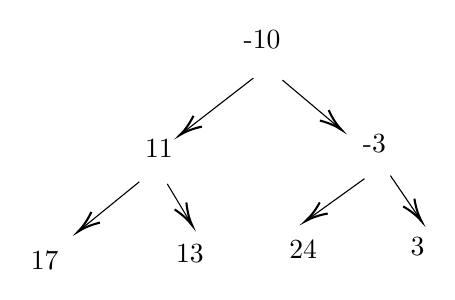
\begin{tikzpicture}[x=0.75pt,y=0.75pt,yscale=-1,xscale=1]
%uncomment if require: \path (0,300); %set diagram left start at 0, and has height of 300

%Straight Lines [id:da17104144614534256] 
\draw    (183.5,64) -- (149.58,90.28) ;
\draw [shift={(148,91.5)}, rotate = 322.24] [color={rgb, 255:red, 0; green, 0; blue, 0 }  ][line width=0.75]    (10.93,-3.29) .. controls (6.95,-1.4) and (3.31,-0.3) .. (0,0) .. controls (3.31,0.3) and (6.95,1.4) .. (10.93,3.29)   ;
%Straight Lines [id:da534935820916556] 
\draw    (197.5,65) -- (224.47,87.71) ;
\draw [shift={(226,89)}, rotate = 220.1] [color={rgb, 255:red, 0; green, 0; blue, 0 }  ][line width=0.75]    (10.93,-3.29) .. controls (6.95,-1.4) and (3.31,-0.3) .. (0,0) .. controls (3.31,0.3) and (6.95,1.4) .. (10.93,3.29)   ;
%Straight Lines [id:da5863622804012776] 
\draw    (128.5,114) -- (100.55,136.74) ;
\draw [shift={(99,138)}, rotate = 320.87] [color={rgb, 255:red, 0; green, 0; blue, 0 }  ][line width=0.75]    (10.93,-3.29) .. controls (6.95,-1.4) and (3.31,-0.3) .. (0,0) .. controls (3.31,0.3) and (6.95,1.4) .. (10.93,3.29)   ;
%Straight Lines [id:da3219044858722526] 
\draw    (142,115) -- (152.97,133.29) ;
\draw [shift={(154,135)}, rotate = 239.04] [color={rgb, 255:red, 0; green, 0; blue, 0 }  ][line width=0.75]    (10.93,-3.29) .. controls (6.95,-1.4) and (3.31,-0.3) .. (0,0) .. controls (3.31,0.3) and (6.95,1.4) .. (10.93,3.29)   ;
%Straight Lines [id:da27448635801952215] 
\draw    (237,112.5) -- (210.12,131.83) ;
\draw [shift={(208.5,133)}, rotate = 324.27] [color={rgb, 255:red, 0; green, 0; blue, 0 }  ][line width=0.75]    (10.93,-3.29) .. controls (6.95,-1.4) and (3.31,-0.3) .. (0,0) .. controls (3.31,0.3) and (6.95,1.4) .. (10.93,3.29)   ;
%Straight Lines [id:da9674312826263478] 
\draw    (249.5,111) -- (263.37,131.35) ;
\draw [shift={(264.5,133)}, rotate = 235.71] [color={rgb, 255:red, 0; green, 0; blue, 0 }  ][line width=0.75]    (10.93,-3.29) .. controls (6.95,-1.4) and (3.31,-0.3) .. (0,0) .. controls (3.31,0.3) and (6.95,1.4) .. (10.93,3.29)   ;

% Text Node
\draw (130,92.5) node [anchor=north west][inner sep=0.75pt]   [align=left] {11};
% Text Node
\draw (235,90) node [anchor=north west][inner sep=0.75pt]   [align=left] {\mbox{-}3};
% Text Node
\draw (199.5,141) node [anchor=north west][inner sep=0.75pt]   [align=left] {24};
% Text Node
\draw (75,146.5) node [anchor=north west][inner sep=0.75pt]   [align=left] {17};
% Text Node
\draw (145,143) node [anchor=north west][inner sep=0.75pt]   [align=left] {13};
% Text Node
\draw (177.5,40) node [anchor=north west][inner sep=0.75pt]   [align=left] {\mbox{-}10};
% Text Node
\draw (258,139.5) node [anchor=north west][inner sep=0.75pt]   [align=left] {3};


\end{tikzpicture}


    \item $[-10, 11, -3, 17, 13, 24, 3]$
    \item Part C
      

\tikzset{every picture/.style={line width=0.75pt}} %set default line width to 0.75pt        

\begin{tikzpicture}[x=0.75pt,y=0.75pt,yscale=-1,xscale=1]
%uncomment if require: \path (0,300); %set diagram left start at 0, and has height of 300

%Straight Lines [id:da17104144614534256] 
\draw    (183.5,64) -- (149.58,90.28) ;
\draw [shift={(148,91.5)}, rotate = 322.24] [color={rgb, 255:red, 0; green, 0; blue, 0 }  ][line width=0.75]    (10.93,-3.29) .. controls (6.95,-1.4) and (3.31,-0.3) .. (0,0) .. controls (3.31,0.3) and (6.95,1.4) .. (10.93,3.29)   ;
%Straight Lines [id:da534935820916556] 
\draw    (197.5,65) -- (224.47,87.71) ;
\draw [shift={(226,89)}, rotate = 220.1] [color={rgb, 255:red, 0; green, 0; blue, 0 }  ][line width=0.75]    (10.93,-3.29) .. controls (6.95,-1.4) and (3.31,-0.3) .. (0,0) .. controls (3.31,0.3) and (6.95,1.4) .. (10.93,3.29)   ;
%Straight Lines [id:da5863622804012776] 
\draw    (128.5,114) -- (100.55,136.74) ;
\draw [shift={(99,138)}, rotate = 320.87] [color={rgb, 255:red, 0; green, 0; blue, 0 }  ][line width=0.75]    (10.93,-3.29) .. controls (6.95,-1.4) and (3.31,-0.3) .. (0,0) .. controls (3.31,0.3) and (6.95,1.4) .. (10.93,3.29)   ;
%Straight Lines [id:da3219044858722526] 
\draw    (136.5,113.5) -- (158.15,137.03) ;
\draw [shift={(159.5,138.5)}, rotate = 227.39] [color={rgb, 255:red, 0; green, 0; blue, 0 }  ][line width=0.75]    (10.93,-3.29) .. controls (6.95,-1.4) and (3.31,-0.3) .. (0,0) .. controls (3.31,0.3) and (6.95,1.4) .. (10.93,3.29)   ;

% Text Node
\draw (128,93) node [anchor=north west][inner sep=0.75pt]   [align=left] {11};
% Text Node
\draw (230.5,91.5) node [anchor=north west][inner sep=0.75pt]   [align=left] {24};
% Text Node
\draw (75,146.5) node [anchor=north west][inner sep=0.75pt]   [align=left] {17};
% Text Node
\draw (155.5,142.5) node [anchor=north west][inner sep=0.75pt]   [align=left] {13};
% Text Node
\draw (183.5,38.5) node [anchor=north west][inner sep=0.75pt]   [align=left] {7};


\end{tikzpicture}


    \item $[7, 11, 24, 17, 13]$
    \item 7
  \end{enumerate}

\end{enumerate}

\newpage

\noindent
\textit{This diagnostic exam will have three portions: a written multiple-choice quiz, a written free-response exam, and a practical implementation problem set. The multiple-choice portion will be timed at only 30 minutes, but you may take as much time as you wish on the free-response and practical portions, provided they are both completed within club hours (before 4:30 PM).}

\noindent
\textit{Answer the following questions to the best of your ability. No points will be removed for incorrect answers, so answer as many as you can. Remember that the purpose of this exam is to guage what you know. This test does not affect your qualification for invitation-only teams, and many of the topics covered on this exam may not have been covered in weekly lectures throughout the year.}

\begin{questions} %------------------------------------------

\section{Multiple Choice Questions}

\fullwidth{\textit{Evaluate the following excerpts of Java source code. This section is intended to test your base knowledge of the Java Standard Programming Language, Version 17. Assume that all necessary class structure, imports, and other preamble information is already in place and that all programs are syntactically correct unless otherwise stated. \\ }}

\begin{minipage}{\textwidth}
\question[1]{What is the value of the expression {\tt 14|11\&9} \\ }

\begin{choices}
  \choice True
  \choice False
  \choice 225
  \choice \textcolor{red}{15}
  \choice 9 \\
\end{choices}
\end{minipage}

By operator precenence, we would do \& before $|$.

\begin{align*}
  11_{10} = 1011_{2}, 9_{10} = 1001_{2} \\
  1011_{2} \& 1001_{2} = 1001_{2} \\
  14_{10} = 1110_{2} \\
  1110_{2} | 1001_{2} = 1111_{2} \\
  1111_{2} = 2^{3} + 2^{2} + 2_{1} + 2^{0} = 15_{10} \\
\end{align*}

% functional programming/streams
\begin{minipage}{\textwidth}
\question[1]{What is the output of this code segment?}

\begin{verbatim}
String[] arr = { "1", "2", "3", "4" };
System.out.println(Arrays.stream(arr)
  .mapToInt(Integer::parseInt)
  .sum());
\end{verbatim}

\begin{choices}
  \choice {\tt 3}
  \choice {\tt 7}
  \choice \textcolor{red}{\tt 10}
  \choice {\tt 4}
  \choice \textit{Error, No Output} \\
\end{choices}
\end{minipage}

The code snippet just converts all of the values in the array to integers then sums them up. $1+2+3+4=10$. \\

\begin{minipage}{\textwidth}
\question[1]{What is the sum of $64_{8}$ and $55_{8}$? \\}

\begin{choices}
  \choice $111_{2}$
  \choice $11001_{2}$
  \choice \textcolor{red}{$1100001_{2}$}
  \choice $111001_{2}$
  \choice $1100111_{2}$ \\
\end{choices}
\end{minipage}

% math.pow question
\begin{minipage}{\textwidth}
\question[1]{Evaluate the following code segment.}

\begin{verbatim}
System.out.println(Math.pow(0x5,02));
\end{verbatim}

\begin{choices}
  \choice {\tt 8.0}
  \choice {\tt 25}
  \choice {\tt 15.0}
  \choice {\tt 0x10}
  \choice \textcolor{red}{\tt 25.0} \\
\end{choices}
\end{minipage}

\begin{enumerate}
  \item {\tt 0x5} is just $5_{16}$, which is equal to $5_{10}$.
  \item {\tt 02} is just $2_{8}$, which is equal to $2_{10}$.
  \item {\tt Math.pow(a,b)} returns a \textit{double} representing $a^{b}$.
\end{enumerate}

Thus, {\tt Math.pow(0x5,02)} is equivalent to $5^{2}$ in float notation.

\begin{minipage}{\textwidth}
\question[1]{Determine the output of the following program excerpt.}

\begin{verbatim}
public int count(String[] data) {
  int result = 0;
  try {
    for (String s: data)
      result += s.length();
  }

  catch (Exception err) {
    result *= -1;
  }

  return result;
}

int v = count(new String[] { "AA", "B", null, "CA", null, "CCC" });
System.out.println(v);

\end{verbatim}

\begin{choices}
  \choice {\tt 0}
  \choice {\tt -1}
  \choice {\tt 3}
  \choice \textcolor{red}{\tt -3}
  \choice {\tt 8} \\
\end{choices}
\end{minipage}

First, it adds the lengths of $v[0]$ and $v[1]$ to result, for a total of 3. Upon hitting $v[2]$, it reaches a NullPointerException for attempting to call a method on a null reference, falls back to the catch block (which simply negates the result counter, leading to $-3$), and returns result.

\begin{minipage}{\textwidth}

\question[1]{Which of the following can replace {\tt $<$*1$>$} in the code segment below so that method {\tt sort(int[], int)} correctly sorts the elements of {\tt data} into ascending order?}

\begin{verbatim}
public void sort(int[] data) {
  sort(data, 0);
}

public void sort(int[] data, int i) {
  if (i < data.length - 1) {
    int j = get_min_index(data, i);
    int temp = data[j];
    data[j] = data[i];
    data[i] = temp;
    <*1>
  }
}

public int get_min_index(int[] data, int i) {
  if (i == data.length - 1)
    return i;
  int j = get_min_index(data, i + 1);
  if (data[i] < data[j])
    return i;
  return j;
}
\end{verbatim}

\begin{enumerate}[label=\Roman*.]
  \item {\tt sort(data, i+1)}
  \item {\tt sort(data, i\textasciicircum2)}
  \item {\tt sort(data, i >> 1)} \\
\end{enumerate}

\begin{choices}
  \choice \textcolor{red}{I only}
  \choice II only
  \choice III only
  \choice I and II
  \choice I, II, and III \\
\end{choices}

II results in stack overflow/infinite recursion by infinitely switching between positions 0 and 2. III results in stack overflow by constantly returning to position 0. Only I will consistently go from position 0 to the full length of the array.

\end{minipage}

% string question

\begin{minipage}{\textwidth}
  \question[1]{What character value denotes the end of a string? (\textit{Hint: NULL}) \\}

\begin{choices}
  \choice \textcolor{red}{0}
  \choice -1
  \choice Character.MAX\_VALUE
  \choice Character.MIN\_VALUE
  \choice 1 \\ 
\end{choices}
\end{minipage}

Strings in Java are null-terminated (a null character denotes the end of the string), and null = 0 \\

% Stacks
\begin{minipage}{\textwidth}
  \question[1]{Stack $S$ contains $[4, 5, 8, 3, 8, 9]$. What would be returned by $pop(S)$ after the following operations (in order): $pop(S)$, $push(S, 10)$, $pop(S)$, $pop(S)$,  and $push(8)$. \textit{Assume that all operations are done to the end of the array-like stack, at position N.} \\ }

\begin{choices}
  \choice 4
  \choice \textcolor{red}{8}
  \choice 3
  \choice 5
  \choice 9 \\
\end{choices}
\end{minipage}

It is a stack, so if the last thing we push is 8, then the next thing we will pop will be 8. \\

% recursion
\begin{minipage}{\textwidth}

\question[1]{Given the definition of method {\tt abc(int)}, What is the output of {\tt abc(0)}?}


\begin{verbatim}
public static int abc(int x) {
  if (x > 10)
    return x - 3;
  else {
    x *= 3;
    return x + abc(x + 2);
  }
}
\end{verbatim}

\begin{choices}
  \choice 51
  \choice 96
  \choice 24
  \choice \textcolor{red}{53}
  \choice 30 \\
\end{choices}

$abc(0) = abc(2) = 53$ \\
$abc(2) = 6 + abc(8) = 6 + 47 = 53$ \\
$abc(8) = 24 + abc(26) = 24 + 23 = 47$ \\
$abc(26) = 23$ \\

\end{minipage}

% code analysis
\begin{minipage}{\textwidth}
\question[1]{What is the output of the following code segment?}

\begin{verbatim}
int number = 20;

switch (number) {
  case 10:
    System.out.println("10");
    break;

  case 20:
    System.out.println("20");

  case 30:
    System.out.println("30");
    break;

  default:
    System.out.println("Not in 10, 20 or 30");
}
\end{verbatim}

\begin{choices}
  \choice \textcolor{red}{\tt 20\\30}
  \choice {\tt 20}
  \choice {\tt 10\\30}
  \choice {\tt 30}
  \choice {\tt Not in 10, 20 or 30} \\
\end{choices}

It begins execution on case 20, printing out {\tt 20}, then falls through to case 30, printing out {\tt 30}. \\

\end{minipage}

% Two's Complement
\begin{minipage}{\textwidth}
\question[1]{Which of the following is the signed 8-bit two's complement representation of $-54$? \\}

\begin{choices}
  \choice $00110110_{2}$
  \choice $11001001_{2}$
  \choice $11001000_{2}$
  \choice $01001001_{2}$
  \choice \textcolor{red}{$11001010_{2}$} \\
\end{choices}

  All two's complement means is that because this is a negative number, we flip all of the bits of its positive version and add 1. $54_{10} = 00110110_{2}$, which flipped is $11001001_{2}$, plus one would be $11001010_{2}$. \\

\end{minipage}

% Binary Search Tree
\begin{minipage}{\textwidth}
\question[1]{After inserting the following values into a binary search tree in order, what is the value of the left-most node? \\ }

90, 20, 66, -2, 393, 8675, 10, 5 \\

\begin{choices}
  \choice \textcolor{red}{$-2$}
  \choice 393
  \choice 5
  \choice 10
  \choice 66 \\
\end{choices}

The leftmost node of a binary search tree is always the minimum value, so this would be -2. \\

\end{minipage}

% Inheritance

\begin{minipage}{\textwidth}
\question[1]{Which of the following class declaration signatures best represents the relationship between animal classes? \\ }

\begin{choices}
    \choice {\tt class Dog extends Feline implements Bark, Meow}
  \choice {\tt class Dog extends Canine implements Meow, Talk}
  \choice \textcolor{red}{\tt class Dog extends Canine implements Bark, Bite}
  \choice {\tt class Dog extends Feline implements Sing, Dance}
  \choice {\tt class Dog implements Mammal, Feline, Reptile} \\
\end{choices}

\end{minipage}

\newpage

\section{Free Response Questions}

\fullwidth{\textit{Read, analyze, and respond to the following questions. These questions may have multiple correct answer choices. This section is intended to test your understanding of applying fundamental competitive programming topics as shown throughout the year.}}

\fullwidth{\textit{Remember, not all of the content covered in any portion of this exam has been covered during a lecture, and this exam is simply to guage how much you each have grown. Simply try your best, and answer as many questions as you can to the best of your ability.}}

\fullwidth{\textit{Unless told otherwise, solve every problem by writing either complete Java code or pseudocode. Make sure to be concise, and avoid writing boilerplate class implementations or input code.}}

% operator precedence

\question[1]{Rank the following operators by precedence: {\tt +}, {\tt $<<$}, {\tt \&}, {\tt |}, {\tt !=}, {\tt /}, {\tt =}, {\tt ++}, {\tt $<$=}, and {\tt \textasciicircum}} \\

Answer: \textcolor{red}{\tt $++$, /, $<<$, $<=$, $!=$, \&, \textasciicircum, |, =} \\

Follow UMBREBLA, see the java operator heirarchy for details. \\

% integer width

\question[8]{Fill in the table for the width of each integer type in both bits and bytes. \\}

\begin{table}[H]
\centering
\begin{tabular}{|l|l|l|}
  \hline
  Type & Bits & Bytes \\ \hline
  boolean & \textcolor{red}{1} & \textcolor{red}{1} \\ \hline
  char & \textcolor{red}{16} & \textcolor{red}{2} \\ \hline
  byte & \textcolor{red}{8} & \textcolor{red}{1} \\ \hline
  short & \textcolor{red}{16} & \textcolor{red}{2} \\ \hline
  int & \textcolor{red}{32} & \textcolor{red}{4} \\ \hline
  long & \textcolor{red}{64} & \textcolor{red}{8} \\ \hline
  float & \textcolor{red}{32} & \textcolor{red}{4} \\ \hline
  double & \textcolor{red}{64} & \textcolor{red}{8} \\ \hline
\end{tabular}
\end{table}

% permutations

\question[2]{Given array $A = [3, 9]$,}

\begin{enumerate}[label=(\Alph*)]
  \item Write every permutation of $A$ that would be generated by an \textit{inconsistent size} permuting algorithm. \\

  \textcolor{red}{$[]$, $[3]$, $[9]$, $[3, 9]$, $[9, 3]$}

\vspace{\stretch{1}}

  \item Write every permutation of $A$ that would be generated by a \textit{consistent size} permuting algorithm. \\
   
  \textcolor{red}{$[3,9]$ and $[9,3]$}

\vspace{\stretch{1}}
\end{enumerate}

% debugging
\begin{minipage}{\textwidth}
  \question[3]{(a) Highlight the error(s) in the following code segment, and explain both (b) why it is an error and (c) what type of error it is (compiler/runtime/logical).}

\begin{verbatim}
public static int hello() {
  int a = 5;
  int b = 8;

  if (a > b) {
    return a;
  }

  else {
    return b;
  }

  return a; <-- (a) This is the problem
}
\end{verbatim}

\begin{enumerate}[label=(\alph*)]
  \addtocounter{enumi}{1}
  \item There is an else statement that returns, so it will never hit the final return statement.
  \item Compiler Error (This will be caught by the compiler, and will prevent the program from running.)
\end{enumerate}

\end{minipage}

% bubble sort question
\question[4]{Write the pseudocode for the Bubble Sort algorithm.}

\begin{verbatim}
function BUBBLESORT(ARRAY)							            
    # loop through the array multiple times
    (1) loop INDEX from 0 to size of ARRAY - 1					    
        # consider every pair of elements except the sorted ones
        (2) loop INDEX2 from 0 to size of ARRAY - 2 - INDEX			
            (3) if ARRAY[INDEX2] > ARRAY[INDEX2 + 1] then			
                (4) # swap elements if they are out of order
                TEMP = ARRAY[INDEX2]						    
                ARRAY[INDEX2] = ARRAY[INDEX2 + 1]				
                ARRAY[INDEX2 + 1] = TEMP					    
\end{verbatim}

% thought question about queues/stacks
\question[2]{Write a class structure with the methods $pop()$ and $push(X)$ that uses only 2 stacks yet emulates a queue's behavior (FIFO)}

\begin{verbatim}
stack A, B

(1) function POP()
  if A is empty
    return nothing or null or -1

  return A.pop()

(2) function PUSH(VALUE)
  while A is not empty
    B.push(A.pop())

  A.push(VALUE)

  while B is not empty
    A.push(B.pop())

\end{verbatim}

% graph theory

\question[8]{Given the following travel index, a list of flights between two destinations run every day alongside the associated cost, answer the following:}

\begin{table}[H]
  \begin{tabular}{p{0.5\textwidth}p{0.5\textwidth}}
\begin{itemize}
  \item Houston $\to$ Austin: \$83
  \item Houston $\to$ Boston: \$534
  \item Houston $\to$ San Antonio: \$68
  \item Austin $\to$ Houston: \$65
  \item Miami $\to$ Boston: \$331
  \item Minneapolis $\to$ Tampa: \$267
  \item San Antonino $\to$ Los Angeles: \$389
  \item Miami $\to$ Houston: \$243
\end{itemize} &
\begin{itemize}
  \item Austin $\to$ Miami: \$124
  \item Portland $\to$ New Orleans: \$637
  \item Boston $\to$ Mineappolis: \$339
  \item Boston $\to$ Miami: \$415
  \item Los Angeles $\to$ Boston: \$382 
  \item Tampa $\to$ Miami: \$43
  \item Miami $\to$ Tampa: \$57
  \item Houston $\to$ Minneapolis: \$143
\end{itemize}
\end{tabular}
\end{table}

\begin{enumerate}[label=(\Alph*)]
  \begin{minipage}{\textwidth}
  \item Draw the graph this travel index represents, including the cost and the directions of each flight.
  

\tikzset{every picture/.style={line width=0.75pt}} %set default line width to 0.75pt        

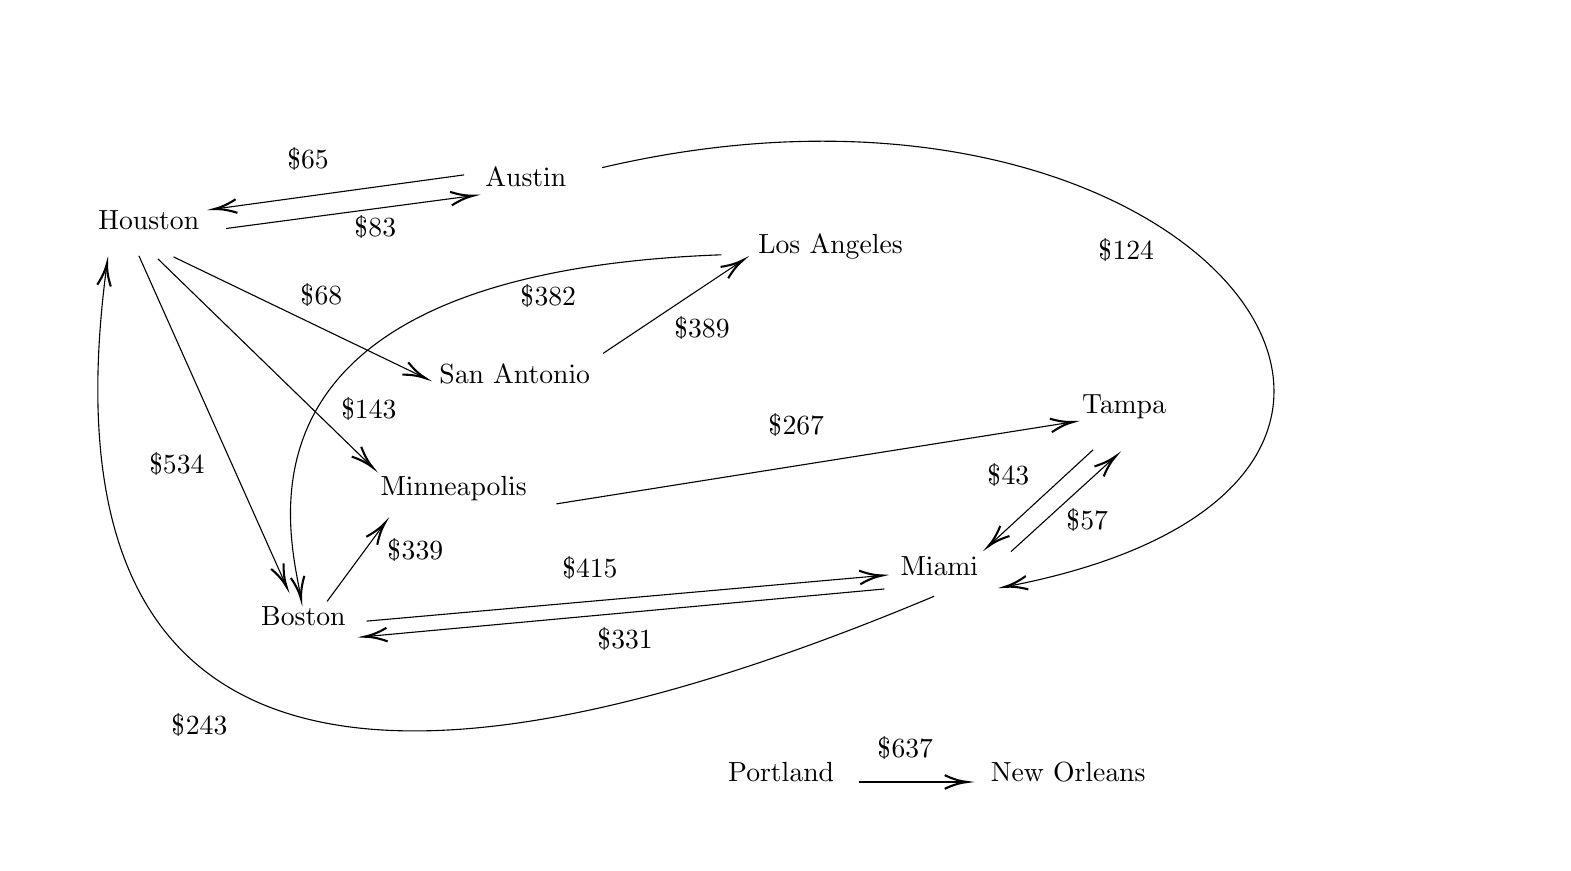
\begin{tikzpicture}[x=0.75pt,y=0.75pt,yscale=-1,xscale=1]
%uncomment if require: \path (0,339); %set diagram left start at 0, and has height of 339

%Straight Lines [id:da5586549096582035] 
\draw    (103,63.5) -- (222.7,121.13) ;
\draw [shift={(224.5,122)}, rotate = 205.71] [color={rgb, 255:red, 0; green, 0; blue, 0 }  ][line width=0.75]    (10.93,-3.29) .. controls (6.95,-1.4) and (3.31,-0.3) .. (0,0) .. controls (3.31,0.3) and (6.95,1.4) .. (10.93,3.29)   ;
%Straight Lines [id:da26174023331430885] 
\draw    (128.33,49.83) -- (245.52,34.26) ;
\draw [shift={(247.5,34)}, rotate = 172.43] [color={rgb, 255:red, 0; green, 0; blue, 0 }  ][line width=0.75]    (10.93,-3.29) .. controls (6.95,-1.4) and (3.31,-0.3) .. (0,0) .. controls (3.31,0.3) and (6.95,1.4) .. (10.93,3.29)   ;
%Straight Lines [id:da2538209687911336] 
\draw    (86.33,63) -- (156.69,220.67) ;
\draw [shift={(157.5,222.5)}, rotate = 245.95] [color={rgb, 255:red, 0; green, 0; blue, 0 }  ][line width=0.75]    (10.93,-3.29) .. controls (6.95,-1.4) and (3.31,-0.3) .. (0,0) .. controls (3.31,0.3) and (6.95,1.4) .. (10.93,3.29)   ;
%Straight Lines [id:da4001782652965149] 
\draw    (243,24) -- (124.48,40.23) ;
\draw [shift={(122.5,40.5)}, rotate = 352.2] [color={rgb, 255:red, 0; green, 0; blue, 0 }  ][line width=0.75]    (10.93,-3.29) .. controls (6.95,-1.4) and (3.31,-0.3) .. (0,0) .. controls (3.31,0.3) and (6.95,1.4) .. (10.93,3.29)   ;
%Straight Lines [id:da041617700111323375] 
\draw    (445.5,223.5) -- (196.99,246.32) ;
\draw [shift={(195,246.5)}, rotate = 354.75] [color={rgb, 255:red, 0; green, 0; blue, 0 }  ][line width=0.75]    (10.93,-3.29) .. controls (6.95,-1.4) and (3.31,-0.3) .. (0,0) .. controls (3.31,0.3) and (6.95,1.4) .. (10.93,3.29)   ;
%Straight Lines [id:da8329943008479503] 
\draw    (506.5,205.5) -- (555.52,160.85) ;
\draw [shift={(557,159.5)}, rotate = 137.67] [color={rgb, 255:red, 0; green, 0; blue, 0 }  ][line width=0.75]    (10.93,-3.29) .. controls (6.95,-1.4) and (3.31,-0.3) .. (0,0) .. controls (3.31,0.3) and (6.95,1.4) .. (10.93,3.29)   ;
%Straight Lines [id:da47224022637364105] 
\draw    (546,156.5) -- (496.97,201.65) ;
\draw [shift={(495.5,203)}, rotate = 317.36] [color={rgb, 255:red, 0; green, 0; blue, 0 }  ][line width=0.75]    (10.93,-3.29) .. controls (6.95,-1.4) and (3.31,-0.3) .. (0,0) .. controls (3.31,0.3) and (6.95,1.4) .. (10.93,3.29)   ;
%Straight Lines [id:da9628050450952343] 
\draw    (287.5,182.5) -- (534.52,143.31) ;
\draw [shift={(536.5,143)}, rotate = 170.99] [color={rgb, 255:red, 0; green, 0; blue, 0 }  ][line width=0.75]    (10.93,-3.29) .. controls (6.95,-1.4) and (3.31,-0.3) .. (0,0) .. controls (3.31,0.3) and (6.95,1.4) .. (10.93,3.29)   ;
%Straight Lines [id:da226264189484929] 
\draw    (95.5,64.5) -- (197.57,163.61) ;
\draw [shift={(199,165)}, rotate = 224.16] [color={rgb, 255:red, 0; green, 0; blue, 0 }  ][line width=0.75]    (10.93,-3.29) .. controls (6.95,-1.4) and (3.31,-0.3) .. (0,0) .. controls (3.31,0.3) and (6.95,1.4) .. (10.93,3.29)   ;
%Straight Lines [id:da6692318860243534] 
\draw    (177,229.5) -- (203.81,193.11) ;
\draw [shift={(205,191.5)}, rotate = 126.38] [color={rgb, 255:red, 0; green, 0; blue, 0 }  ][line width=0.75]    (10.93,-3.29) .. controls (6.95,-1.4) and (3.31,-0.3) .. (0,0) .. controls (3.31,0.3) and (6.95,1.4) .. (10.93,3.29)   ;
%Straight Lines [id:da3695263760558307] 
\draw    (310,110) -- (375.84,66.11) ;
\draw [shift={(377.5,65)}, rotate = 146.31] [color={rgb, 255:red, 0; green, 0; blue, 0 }  ][line width=0.75]    (10.93,-3.29) .. controls (6.95,-1.4) and (3.31,-0.3) .. (0,0) .. controls (3.31,0.3) and (6.95,1.4) .. (10.93,3.29)   ;
%Curve Lines [id:da8778567739345868] 
\draw    (469.5,227) .. controls (243,322) and (33,345.5) .. (71,66.5) ;
\draw [shift={(71,66.5)}, rotate = 97.76] [color={rgb, 255:red, 0; green, 0; blue, 0 }  ][line width=0.75]    (10.93,-3.29) .. controls (6.95,-1.4) and (3.31,-0.3) .. (0,0) .. controls (3.31,0.3) and (6.95,1.4) .. (10.93,3.29)   ;
%Straight Lines [id:da5372204427280081] 
\draw    (196,239) -- (442.51,217.18) ;
\draw [shift={(444.5,217)}, rotate = 174.94] [color={rgb, 255:red, 0; green, 0; blue, 0 }  ][line width=0.75]    (10.93,-3.29) .. controls (6.95,-1.4) and (3.31,-0.3) .. (0,0) .. controls (3.31,0.3) and (6.95,1.4) .. (10.93,3.29)   ;
%Curve Lines [id:da14992676931134008] 
\draw    (507.38,221.75) .. controls (762.33,171.3) and (596.06,-46.66) .. (309.5,20.5) ;
\draw [shift={(503.5,222.5)}, rotate = 349.35] [color={rgb, 255:red, 0; green, 0; blue, 0 }  ][line width=0.75]    (10.93,-3.29) .. controls (6.95,-1.4) and (3.31,-0.3) .. (0,0) .. controls (3.31,0.3) and (6.95,1.4) .. (10.93,3.29)   ;
%Curve Lines [id:da6295751604837766] 
\draw    (164.1,226.18) .. controls (158.16,193.65) and (125.69,71.28) .. (367,62.5) ;
\draw [shift={(164.5,228.5)}, rotate = 261.03] [color={rgb, 255:red, 0; green, 0; blue, 0 }  ][line width=0.75]    (10.93,-3.29) .. controls (6.95,-1.4) and (3.31,-0.3) .. (0,0) .. controls (3.31,0.3) and (6.95,1.4) .. (10.93,3.29)   ;
%Straight Lines [id:da2183394977689802] 
\draw    (433.5,316.5) -- (483.5,316.5) ;
\draw [shift={(485.5,316.5)}, rotate = 180] [color={rgb, 255:red, 0; green, 0; blue, 0 }  ][line width=0.75]    (10.93,-3.29) .. controls (6.95,-1.4) and (3.31,-0.3) .. (0,0) .. controls (3.31,0.3) and (6.95,1.4) .. (10.93,3.29)   ;

% Text Node
\draw (65.5,40) node [anchor=north west][inner sep=0.75pt]   [align=left] {Houston};
% Text Node
\draw (252,19) node [anchor=north west][inner sep=0.75pt]   [align=left] {Austin};
% Text Node
\draw (229.83,114) node [anchor=north west][inner sep=0.75pt]   [align=left] {San Antonio};
% Text Node
\draw (144,230.67) node [anchor=north west][inner sep=0.75pt]   [align=left] {Boston};
% Text Node
\draw (90,156.67) node [anchor=north west][inner sep=0.75pt]   [align=left] {\$534};
% Text Node
\draw (163,75) node [anchor=north west][inner sep=0.75pt]   [align=left] {\$68};
% Text Node
\draw (189,42.5) node [anchor=north west][inner sep=0.75pt]   [align=left] {\$83};
% Text Node
\draw (156.5,9.5) node [anchor=north west][inner sep=0.75pt]   [align=left] {\$65};
% Text Node
\draw (452,206.5) node [anchor=north west][inner sep=0.75pt]   [align=left] {Miami};
% Text Node
\draw (306,241) node [anchor=north west][inner sep=0.75pt]   [align=left] {\$331};
% Text Node
\draw (539.5,128.5) node [anchor=north west][inner sep=0.75pt]   [align=left] {Tampa};
% Text Node
\draw (494,162) node [anchor=north west][inner sep=0.75pt]   [align=left] {\$43};
% Text Node
\draw (532,183.5) node [anchor=north west][inner sep=0.75pt]   [align=left] {\$57};
% Text Node
\draw (201.5,168) node [anchor=north west][inner sep=0.75pt]   [align=left] {Minneapolis};
% Text Node
\draw (388.5,138) node [anchor=north west][inner sep=0.75pt]   [align=left] {\$267};
% Text Node
\draw (182.5,130) node [anchor=north west][inner sep=0.75pt]   [align=left] {\$143};
% Text Node
\draw (205,198) node [anchor=north west][inner sep=0.75pt]   [align=left] {\$339};
% Text Node
\draw (383.5,51.5) node [anchor=north west][inner sep=0.75pt]   [align=left] {Los Angeles};
% Text Node
\draw (343,91) node [anchor=north west][inner sep=0.75pt]   [align=left] {\$389};
% Text Node
\draw (101,282.5) node [anchor=north west][inner sep=0.75pt]   [align=left] {\$243};
% Text Node
\draw (289,206.5) node [anchor=north west][inner sep=0.75pt]   [align=left] {\$415};
% Text Node
\draw (547.5,53.5) node [anchor=north west][inner sep=0.75pt]   [align=left] {\$124};
% Text Node
\draw (269,75.5) node [anchor=north west][inner sep=0.75pt]   [align=left] {\$382};
% Text Node
\draw (369,305.5) node [anchor=north west][inner sep=0.75pt]   [align=left] {Portland};
% Text Node
\draw (495.5,305.5) node [anchor=north west][inner sep=0.75pt]   [align=left] {New Orleans};
% Text Node
\draw (441,293.5) node [anchor=north west][inner sep=0.75pt]   [align=left] {\$637};


\end{tikzpicture}


  \end{minipage}

  \item Circle all of the following characteristics that represent this graph.

  \begin{itemize}
    \item \textcolor{red}{Cyclical}/Acyclical
    \item \textcolor{red}{Weighted}/Unweighted
    \item \textcolor{red}{Directed}/Undirected \\
  \end{itemize}

  \item What part of a graph do the places represent? \\ 

  \textcolor{red}{Nodes/Vertices} \\

  \item What part of a graph do the flights represent?  \\

  \textcolor{red}{Edges/Connections/Sides} \\

  \item What would be the traversal order of a Depth-First-Search algorithm that picks places in alphabetical order by name (without consideration to cost) beginning at Houston? \\

  \textcolor{red}{Houston, Austin, Miami, Boston, Minneapolis, Tampa, San Antonio, Los Angeles} \\

  \item (i) What is the cheapest flight path between Tampa and Boston, and (ii) how much does it cost? \\

    \begin{enumerate}[label=(\alph*)]
      \item \textcolor{red}{Boston $\to$ Miami $\to$ Tampa}
      \item \textcolor{red}{\$458}
    \end{enumerate}
\end{enumerate}

\newpage

% Priority Queues
\question[5]{The values $[23_{4}, -3_{5}, 18_{16}, 19_{8}, 1101_{2}, -10_{10}, 11_{2}]$ are inserted into a Priority
Queue $Q$ in order. \textit{Write all values as their base 10 forms.}}

\begin{enumerate}[label=(\Alph*)]
  \item Draw the current state of $Q$ in tree form. \\

    \textcolor{red}{The values converted to base 10 are $[11, -3, 24, 17, 13, -10, 3]$} \\

    

\tikzset{every picture/.style={line width=0.75pt}} %set default line width to 0.75pt        

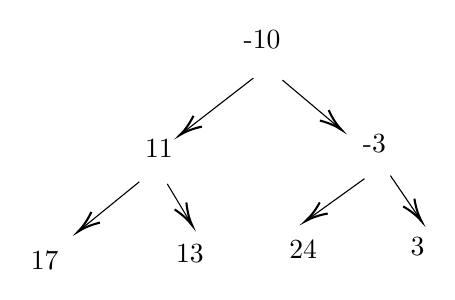
\begin{tikzpicture}[x=0.75pt,y=0.75pt,yscale=-1,xscale=1]
%uncomment if require: \path (0,300); %set diagram left start at 0, and has height of 300

%Straight Lines [id:da17104144614534256] 
\draw    (183.5,64) -- (149.58,90.28) ;
\draw [shift={(148,91.5)}, rotate = 322.24] [color={rgb, 255:red, 0; green, 0; blue, 0 }  ][line width=0.75]    (10.93,-3.29) .. controls (6.95,-1.4) and (3.31,-0.3) .. (0,0) .. controls (3.31,0.3) and (6.95,1.4) .. (10.93,3.29)   ;
%Straight Lines [id:da534935820916556] 
\draw    (197.5,65) -- (224.47,87.71) ;
\draw [shift={(226,89)}, rotate = 220.1] [color={rgb, 255:red, 0; green, 0; blue, 0 }  ][line width=0.75]    (10.93,-3.29) .. controls (6.95,-1.4) and (3.31,-0.3) .. (0,0) .. controls (3.31,0.3) and (6.95,1.4) .. (10.93,3.29)   ;
%Straight Lines [id:da5863622804012776] 
\draw    (128.5,114) -- (100.55,136.74) ;
\draw [shift={(99,138)}, rotate = 320.87] [color={rgb, 255:red, 0; green, 0; blue, 0 }  ][line width=0.75]    (10.93,-3.29) .. controls (6.95,-1.4) and (3.31,-0.3) .. (0,0) .. controls (3.31,0.3) and (6.95,1.4) .. (10.93,3.29)   ;
%Straight Lines [id:da3219044858722526] 
\draw    (142,115) -- (152.97,133.29) ;
\draw [shift={(154,135)}, rotate = 239.04] [color={rgb, 255:red, 0; green, 0; blue, 0 }  ][line width=0.75]    (10.93,-3.29) .. controls (6.95,-1.4) and (3.31,-0.3) .. (0,0) .. controls (3.31,0.3) and (6.95,1.4) .. (10.93,3.29)   ;
%Straight Lines [id:da27448635801952215] 
\draw    (237,112.5) -- (210.12,131.83) ;
\draw [shift={(208.5,133)}, rotate = 324.27] [color={rgb, 255:red, 0; green, 0; blue, 0 }  ][line width=0.75]    (10.93,-3.29) .. controls (6.95,-1.4) and (3.31,-0.3) .. (0,0) .. controls (3.31,0.3) and (6.95,1.4) .. (10.93,3.29)   ;
%Straight Lines [id:da9674312826263478] 
\draw    (249.5,111) -- (263.37,131.35) ;
\draw [shift={(264.5,133)}, rotate = 235.71] [color={rgb, 255:red, 0; green, 0; blue, 0 }  ][line width=0.75]    (10.93,-3.29) .. controls (6.95,-1.4) and (3.31,-0.3) .. (0,0) .. controls (3.31,0.3) and (6.95,1.4) .. (10.93,3.29)   ;

% Text Node
\draw (130,92.5) node [anchor=north west][inner sep=0.75pt]   [align=left] {11};
% Text Node
\draw (235,90) node [anchor=north west][inner sep=0.75pt]   [align=left] {\mbox{-}3};
% Text Node
\draw (199.5,141) node [anchor=north west][inner sep=0.75pt]   [align=left] {24};
% Text Node
\draw (75,146.5) node [anchor=north west][inner sep=0.75pt]   [align=left] {17};
% Text Node
\draw (145,143) node [anchor=north west][inner sep=0.75pt]   [align=left] {13};
% Text Node
\draw (177.5,40) node [anchor=north west][inner sep=0.75pt]   [align=left] {\mbox{-}10};
% Text Node
\draw (258,139.5) node [anchor=north west][inner sep=0.75pt]   [align=left] {3};


\end{tikzpicture}



  \item Draw the current state of $Q$ in array form. \\

  \textcolor{red}{$[-10, 11, -3, 17, 13, 24, 3]$} \\

\end{enumerate}

The following operations are performed on $A$ in the following order: $pop(Q)$, $pop(Q)$, $pop(Q)$, $push(Q, 13_{4})$,
$push(Q, 10_{2} >> 2)$, $push(Q, -8_{16})$, $pop(Q)$, $pop(Q)$ \\

\begin{enumerate}[resume,label=(\Alph*)]
  \item Draw the new state of $Q$ in tree form.

  \textcolor{red}{$-8_{16} = -8_{10}$}

  

\tikzset{every picture/.style={line width=0.75pt}} %set default line width to 0.75pt        

\begin{tikzpicture}[x=0.75pt,y=0.75pt,yscale=-1,xscale=1]
%uncomment if require: \path (0,300); %set diagram left start at 0, and has height of 300

%Straight Lines [id:da17104144614534256] 
\draw    (183.5,64) -- (149.58,90.28) ;
\draw [shift={(148,91.5)}, rotate = 322.24] [color={rgb, 255:red, 0; green, 0; blue, 0 }  ][line width=0.75]    (10.93,-3.29) .. controls (6.95,-1.4) and (3.31,-0.3) .. (0,0) .. controls (3.31,0.3) and (6.95,1.4) .. (10.93,3.29)   ;
%Straight Lines [id:da534935820916556] 
\draw    (197.5,65) -- (224.47,87.71) ;
\draw [shift={(226,89)}, rotate = 220.1] [color={rgb, 255:red, 0; green, 0; blue, 0 }  ][line width=0.75]    (10.93,-3.29) .. controls (6.95,-1.4) and (3.31,-0.3) .. (0,0) .. controls (3.31,0.3) and (6.95,1.4) .. (10.93,3.29)   ;
%Straight Lines [id:da5863622804012776] 
\draw    (128.5,114) -- (100.55,136.74) ;
\draw [shift={(99,138)}, rotate = 320.87] [color={rgb, 255:red, 0; green, 0; blue, 0 }  ][line width=0.75]    (10.93,-3.29) .. controls (6.95,-1.4) and (3.31,-0.3) .. (0,0) .. controls (3.31,0.3) and (6.95,1.4) .. (10.93,3.29)   ;
%Straight Lines [id:da3219044858722526] 
\draw    (136.5,113.5) -- (158.15,137.03) ;
\draw [shift={(159.5,138.5)}, rotate = 227.39] [color={rgb, 255:red, 0; green, 0; blue, 0 }  ][line width=0.75]    (10.93,-3.29) .. controls (6.95,-1.4) and (3.31,-0.3) .. (0,0) .. controls (3.31,0.3) and (6.95,1.4) .. (10.93,3.29)   ;

% Text Node
\draw (128,93) node [anchor=north west][inner sep=0.75pt]   [align=left] {11};
% Text Node
\draw (230.5,91.5) node [anchor=north west][inner sep=0.75pt]   [align=left] {24};
% Text Node
\draw (75,146.5) node [anchor=north west][inner sep=0.75pt]   [align=left] {17};
% Text Node
\draw (155.5,142.5) node [anchor=north west][inner sep=0.75pt]   [align=left] {13};
% Text Node
\draw (183.5,38.5) node [anchor=north west][inner sep=0.75pt]   [align=left] {7};


\end{tikzpicture}



  \item Draw the new state of $Q$ in array form. \\

  \textcolor{red}{$[7, 11, 24, 17, 13]$} \\

  \item What value would be returned by another call of $pop(Q)$? \\

  \textcolor{red}{7}

\end{enumerate}

\newpage


\section{Personal Questions}

\fullwidth{\textit{These questions are simply for us officers (namely Mufaro) to understand how to best serve the computer science club in the future and self-evaluate our performance in training the rest of the club. This section will not count towards your score. \\ }}

\question{How strongly, on a scale of 1 to 10 (10 being the strongest) has your understanding of computer science (in general) improved as a result of your participation in the competitive computer science club this year? \\}

State your reasoning for this score. \\

\vspace{\stretch{1}}

\question{What was the most useful/best thing(s) that was done/offered in through the computer science club that helped you understand competitive computer science? \\}

\vspace{\stretch{1}}

\question{What criticisms/suggestions do you have for the current curriculum/club? \\}

\vspace{\stretch{1}}

\question{Consider what you were intending to major/specialize in during your college/career at the beginning of the year. (a) What was it before, (b) what is it now, and (c) has it changed?}

\vspace{\stretch{1}}

\question{Is there anything else that you would like to tell us? \\}

\vspace{\stretch{1}}

\end{questions}
\end{document}
